\documentclass[10pt]{beamer}

\usetheme[progressbar=frametitle]{metropolis}
\usepackage{appendixnumberbeamer}
\usepackage[numbers,sort&compress]{natbib}
\bibliographystyle{plainnat}

\usepackage{booktabs}
\usepackage[scale=2]{ccicons}
% \usepackage{algorithm, algorithmic}
\usepackage{xspace}
\newcommand{\themename}{\textbf{\textsc{metropolis}}\xspace}

\setbeamercolor{block body}{bg=mDarkTeal!30}
\setbeamercolor{block title}{bg=mDarkTeal,fg=black!2}

\setbeamertemplate{footline}[frame number]
\setbeamertemplate{navigation symbols}{}
\setbeamertemplate{itemize item}[default]
\usepackage{amsmath,amssymb}
\usepackage{braket}
\usepackage{algorithm}
\usepackage[noend]{algpseudocode}
\newcommand{\Hi}{\mathcal{H}}
\newcommand{\eps}{\varepsilon}
\newcommand{\bigket}[1]{\left |#1 \right \rangle}
\newcommand{\bigbra}[1]{\left \langle#1 \right|}
\newcommand{\ip}[2]{\langle #1 | #2 \rangle}
\newcommand{\ipc}[2]{\langle #1 , #2 \rangle}
\newcommand{\ketbra}[2]{|#1\rangle\! \langle #2|}
%\newcommand{\braket}[3]{\langle #1|#3 \rangle}
\newcommand{\braketbra}[3]{\langle #1|#2| #3 \rangle}
\newcommand{\nrm}[1]{\left\lVert #1 \right\rVert}
\newcommand{\bigO}[1]{\mathcal{O}\left( #1 \right)}
\newcommand{\bigObig}[1]{\mathcal{O}\big( #1 \big)}
\newcommand{\bigOt}[1]{\widetilde{\mathcal{O}}\left( #1 \right)}
\newcommand{\phaseO}[1]{\mathrm{O}_{\!#1}}
\newcommand{\phaseOt}[1]{\widetilde{\mathrm{O}}_{\!#1}}
\newcommand{\erf}[1]{\mathrm{erf}\left( #1 \right)}
\newcommand{\erfa}[1]{\mathrm{erfa}\left( #1 \right)}
\newcommand{\erfc}[1]{\mathrm{erfc}\left( #1 \right)}
\newcommand{\sign}[1]{\mathrm{sign}\left( #1 \right)}
\newcommand{\diag}[1]{\mathrm{diag}\left( #1 \right)}
\DeclareMathOperator{\arccosh}{arccosh}
\newcommand{\vertiii}[1]{{\left\vert\kern-0.25ex\left\vert\kern-0.25ex\left\vert #1 
		\right\vert\kern-0.25ex\right\vert\kern-0.25ex\right\vert}}
		
\usepackage[top=2cm, bottom = 2cm, left=2.2cm, right=2.2cm]{geometry}
%special symbols
\newcommand{\C}{\mathbb{C}}
\newcommand{\N}{\mathbb{N}}
\newcommand{\R}{\mathbb{R}}
\newcommand{\Z}{\mathbb{Z}}
\newcommand{\PM}{\mathcal{P}}


%\usepackage{MnSymbol}
\newcommand{\cupdot}{\overset{.}{\cup}}
\newcommand{\pvp}{\vec{p}{\kern 0.45mm}'}
\let\oldnabla\nabla
\renewcommand{\nabla}{\oldnabla\!}

\def\Id{\mathrm{Id}}
\def\polylog{\mathrm{polylog}}
% \def\AND{\mathrm{AND}}
\def\Pr{\mathrm{Pr}}
\def\Tr{\mathrm{Tr}}
\def\im{\mathrm{im}}

\providecommand{\trnorm}[1]{\left\lVert#1\right\rVert_1}
\providecommand{\infnorm}[1]{\left\lVert#1\right\rVert_{\infty}}
\providecommand{\spnorm}[1]{\left\lVert#1\right\rVert}
\providecommand{\maxnorm}[1]{\left\lVert#1\right\rVert_{\max}}
\providecommand{\tr}[1]{\Tr\left[#1\right]}
\providecommand{\sgn}[1]{\mathrm{sgn}\left(#1\right)}
\providecommand{\rank}[1]{\mathrm{rank}\left(#1\right)}
\providecommand{\poly}[1]{\mathrm{poly}\left(#1\right)}
\providecommand{\img}[1]{\mathrm{img}\left(#1\right)}
\providecommand{\spn}[1]{\mathrm{Span}\left(#1\right)}
\providecommand{\eend}[1]{\mathrm{End}\left(#1\right)}

\long\def\ignore#1{}

\usepackage{tikz,pgfplots}

%%%% User commands for Section 2 / 3
\newcommand\lr[1]{\left( #1 \right)}
\newcommand\lrv[1]{\left|  #1 \right|}
\newcommand\lrb[1]{\left\lbrace #1 \right\rbrace}
\newcommand{\smallO}[1]{ {o}\left( #1 \right)}
% For Section 3:
\renewcommand{\check}{\mathtt{Check}}
\newcommand{\setup}{\mathtt{Setup}}
\newcommand{\update}{\mathtt{Update}}
\newcommand{\checkingcost}{\mathsf{C}}
\newcommand{\setupcost}{\mathsf{S}}
\newcommand{\updatecost}{\mathsf{U}}
\newcommand{\Reg}{\mathsf{R}}
\newcommand{\barO}{\bar{0}}
\newcommand{\psuccess} {p_{\textrm{success}}}
\newtheorem{exmp}{Example}[section]


\title{Quantum walks and application to search problems}
\author{Krishna Acharya}
\date{January 2020}

\begin{document}
\maketitle

\begin{frame}{Overview}
\tableofcontents
\end{frame}

\section{Random walks on a Line}
\begin{frame}{Introduction}
    \begin{itemize}
        \item Consider a line, with grid-length $1$ and a particle starting off at $x=0$
        \item The probability of moving left or right is $\frac{1}{2}$
        \item  
         \begin{figure}[H]
         \centering
         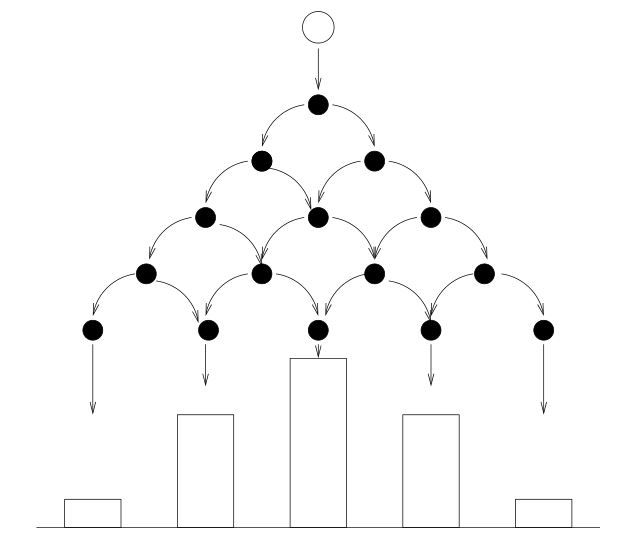
\includegraphics[width=60mm]{Images/Galton.JPG}
         \caption{Classical distribution}
        \end{figure}
    \end{itemize}
\end{frame}
\begin{frame}{Quantum walk on a line}
    \begin{itemize}
        \item The basis states for $\Hi_P$  are $\{\ket{i}: i\in \mathbb{Z}\}$
        \item A coin space $\Hi_C$ augments $\Hi_P$, basis states for which are $\{\ket{left}, \ket{right} \}$. State for the total system $\Hi = \Hi_C \otimes \Hi_P$
        \item The conditional shift operator $S$, transforms $\ket{left} \otimes \ket{i}$ to  $\ket{left} \otimes \ket{i-1}$ and $\ket{right} \otimes \ket{i}$ to  $\ket{right} \otimes \ket{i+1}$
        \item Equivalently $S = \sum_i{\ket{right} \otimes \ket{i+1} \bra{right}\otimes\bra{i}} + \sum_i{\ket{left} \otimes \ket{i-1} \bra{left}\otimes\bra{i}}$
    \end{itemize}
\end{frame}

\begin{frame}{The Unitary}
    \begin{itemize}
        \item Quantum walk for $t$ steps is given by $U^t$, where $U = S \cdot (C \otimes I)$
        \item Coin flip acts just on $\Hi_C$, The choice for the coin is:
        \begin{equation*}
            C = \frac{1}{\sqrt{2}}
            \begin{pmatrix}
            1 & i \\
            i & 1
            \end{pmatrix}
        \end{equation*}
     \item For the starting state $\ket{left}\ket{0} \xrightarrow{S \cdot (C\otimes I)} \frac{1}{\sqrt{2}}\ket{right}\ket{1} + \frac{i}{\sqrt{2}} \ket{left}\ket{-1}$
    \end{itemize}
\end{frame}

\begin{frame}{Distribution Comparison}
    \begin{figure}
\centering
\begin{minipage}{.5\textwidth}
  \centering
  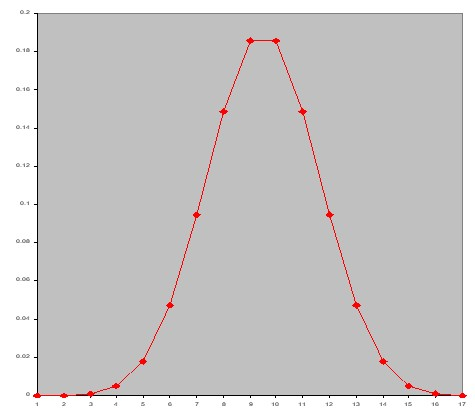
\includegraphics[width=0.95\linewidth]{Images/ClassicalLRwalk.jpg}
  \label{fig:test1}
\end{minipage}%
\begin{minipage}{.5\textwidth}
  \centering
  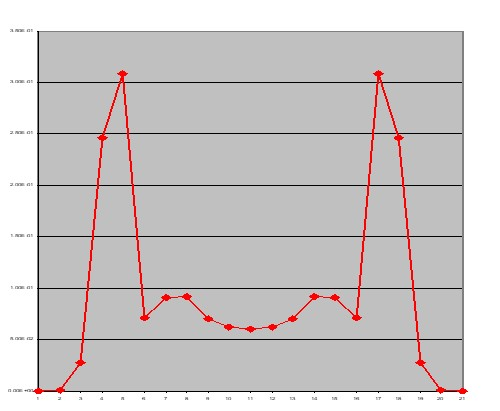
\includegraphics[width=0.95\linewidth]{Images/QuantumLRwalk.jpg}
  \label{fig:test2}
\end{minipage}
\end{figure}
\begin{itemize}
    \item Classical walk after $T$ steps has a $\sigma = \Theta(\sqrt{T})$ whereas quantum walk has $\sigma = \Theta({T})$
    \item Quadratically faster propogation.
\end{itemize}
\end{frame}
\section{Quantum walk for database search}
\begin{frame}{Quantum walk search algorithm}
    \begin{itemize}
        \item Search space : $n$-bit binary strings, $x \in \{0,1\}^n$
        \item $f(\vec{x}) \in \{0,1\}$ is such that $f(x) = 1$ for exactly one input $\vec{x}_{target}$
        \item Goal: Find $\vec{x}_{target}$ 
        \item Using the mapping of n-bit binary string to nodes on the hypercube, the search problem is then equivalent to searching for a single marked node amongst the $N = 2^n$ nodes.
    \end{itemize}
\end{frame}

\begin{frame}{Shift and Coin operators}

    \begin{itemize}
        \item $\ket{d, \vec{x}} \xrightarrow{S} \ket{d, \vec{x} \oplus \vec{e_d}}$
            \begin{equation}
            S = \sum_{d=0}^{n-1}{\sum_{\vec{x}}{
            \ket{d, \vec{x} \oplus \vec{e_d}}\bra{d, \vec{x}}}}    
        \end{equation}
        \item The coin operator to be applied is perturbed, 
        \begin{equation}
            C_{pert} = C_0 \otimes I - \left(I +
            C_0\right)\otimes\ket{\vec{0}}\bra{\vec{0}}.
        \end{equation}
    \end{itemize}
    
    \begin{algorithm}[H]
    \caption{Search with coin oracle}\label{alg:q1}
    \begin{algorithmic}[1]
    \Procedure{Find Marked}{} %\Comment{The g.c.d. of a and b}
    \State $\psi_0 \gets \ket{s^C} \otimes \ket{s^S}$ i.e equal superposition over all states
    \State Compute $U_{pert}^t \ket{\psi_0}$ where $t =\frac{\pi}{2}\sqrt{2^n}$
    \State Measure in $\ket{d,\vec{x}}$ basis
    \EndProcedure
    \end{algorithmic}
    \end{algorithm}
\end{frame}

\begin{frame}{Outcome on measurement}
    \begin{itemize}
        \item Wp $\frac{1}{2} - O(1/n)$, the measured outcome is the marked state.
        \item The proof for the earlier algorithm: is that the walk can be \textit{approximately} mapped onto a 2D subspace.
        % \item Unlike Grover search, the final state is not exactly the pure marked state $\ket{0}$ but also has small contributions from its nearest neighbours.
        \item The approximations for the initial state and final state are $\pi/2$ apart and each application of $U$ corresponds to a rotation angle of $1/\sqrt{2^{n-1}}$. So the search is completed after $\frac{\pi}{2} \sqrt{2^{n-1}}$ steps.
        \item Running time is $\bigO{\sqrt{N}}$
    \end{itemize}
\end{frame}
\section{Quantum walk for Spatial search}
\begin{frame}{Spatial search, Quadratic speedup for finding marked vertices}
    \begin{itemize}
        \item Finding a marked vertex in a general graph, when multiple marked vertices exist was an open problem.
        \item Ambainis et al find an  $\bigOt{\sqrt{HT}}$ algorithm.
        \item Key components for this result are \textbf{Interpolated walk} and \textbf{Quantum fast forwarding} this walk.
    \end{itemize}
\end{frame}

\begin{frame}{Ergodic chain, Discriminant Matrix}
\begin{itemize}
    \item $\PM$ is \emph{ergodic} if for a large enough $t\in \N$ all elements of $\PM^t$ are non-zero. 
    \item The corresponding \emph{time-reversed} Markov chain is defined as $\PM^*:=\diag{\pi}^{-1}\cdot\PM^T\cdot\diag{\pi}$.  $\PM$ is \emph{reversible} if it is ergodic and $\PM^*=\PM$.
    \item Discriminant matrix $D$'s $xy$-entry is $\sqrt{\PM_{xy}\PM^*_{yx}}$.
        \begin{equation}\label{eq:discriminant}
        D=\diag{\pi}^{\frac12}\cdot\PM\cdot\diag{\pi}^{-\frac12}.
        \end{equation}
        \end{itemize}

\end{frame}

\begin{frame}{Interpolated walk}
\begin{itemize}
    \item For $\PM$ the marked set $M\subset X$. ~~ $\PM'$ is the absorbing markov chain.
        \begin{align*}
    \PM :=\left(\begin{array}{cc} \PM_{UU} & \PM_{UM} \\ \PM_{MU} & \PM_{MM} \end{array}\right), & &
    \PM' :=\left(\begin{array}{cc} \PM_{UU} & \PM_{UM} \\ 0 & I \end{array}\right).
    \end{align*}
    \item The \emph{interpolated walk} operator, for $s\in [0,1)$:
$\PM(s):=(1 - s)\PM + s\PM'$
\end{itemize}
\end{frame}

\begin{frame}{Quantum Fast forwarding}
The following result is by Apers and Sarlette:
    \begin{theorem}\label{thm:fast-forwarding}
Let $\eps\in(0,1)$, $s\in[0,1]$ and $t\in\mathbb{N}$. Let $\cal P$ be any reversible Markov chain on state space $X$, and let $\mathsf{Q}$ be the cost of implementing the (controlled) quantum walk operator $W(s)$. There is a quantum algorithm with complexity $\bigO{\sqrt{t\log(1/\eps)}\mathsf{Q}}$ that takes input $\ket{\barO}\ket{\psi}\in \mathrm{span}\{\ket{\barO}\ket{x}:x\in X\}$, and outputs a state that is $\eps$-close to a state of the form
$$\ket{0}^{\!\otimes a}\ket{\barO}D^t\ket{\psi}+\ket{\Gamma}$$
where $a=\bigO{\log(t\log(1/\eps))}$ and $\ket{\Gamma}$ is some garbage state that has no support on states containing $\ket{0}^{\!\otimes a}\ket{\barO}$ in the first two registers.%, and $\nrm{\ket{\Gamma}}^2 = 1 - \nrm{D^t\ket{\psi}}^2$ (which may depend on $\ket{\psi}$ and $t$). 
\end{theorem}
\end{frame}

\begin{frame}{Main result by Ambainis et al}
    \begin{theorem}
	Let $\cal P$ be a reversible ergodic Markov chain, and let $\pi$ be its stationary distribution.
	If $p_M\leq 1/9$ and $T\geq 3HT$, then choosing $s\in S=\{1-\frac{1}{r}:r\in R\}$ and $t\in [24T]$ uniformly at random we get, that 
	$$\mathbb{E}\left[\nrm{\Pi_M D^t(s)\ket{\sqrt{\pi_U}}}^2\right]= \Omega\left(\frac{1}{\log(T)}\right).$$
\end{theorem}\label{cor:AMRMS}
\end{frame}

\begin{frame}[shrink]{FF-based search}

\begin{algorithm}[H]
	\textbf{Search}($ \PM $, $ M $, $T$)\\ %: aim
	Use $\bigO{\!\!\sqrt{\log(T)}}\!$ rounds amplitude amplification to amplify the success probability of steps~1-$3$:
	\begin{enumerate}
		\item Use $\setup(\PM)$ to prepare the state $$\sum_{t=1}^{T}\frac{1}{\sqrt{T}}\ket{t}\sum_{s\in S}\frac{1}{\sqrt{|S|}}\ket{s}\ket{\sqrt{\pi}}.$$
		\item Measure $\{\Pi_M,I-\Pi_M\}$ on the last register. If the outcome is ``marked'', measure in the computational basis, and output the entry in the last register. Otherwise continue with the (subnormalized) post-measurement state %\frac{1}{\sqrt{1-p_M}}
		$$\sum_{t=1}^{T}\frac{1}{\sqrt{T}}\ket{t}\sum_{s\in S}\frac{1}{\sqrt{|S|}}\ket{s}\ket{\sqrt{\pi_U}}.$$
		\item Use quantum fast-forwarding, controlled on the first two registers, to map $\ket{t}\ket{s}\ket{\sqrt{\pi_U}}$ to $\ket{1}\ket{t}\ket{s}D^t(s)\ket{\pi_U}+\ket{0}\ket{\Gamma}$ for some arbitrary $\ket{\Gamma}$, with precision $\bigO{\frac{1}{\log(T)}}$. Finally, measure the last register and output its content if marked, otherwise output \texttt{No marked vertex}.
	\end{enumerate}
	\caption{Fast-forwarding-based search algorithm}\label{alg:alg2}
\end{algorithm}
\end{frame}

\begin{frame}{Runtime}
The complexity of steps 1-3 is
$\bigO{\mathsf{S}+\sqrt{T\log\log(T)}(\mathsf{U}+\mathsf{C})}$
Amplitude amplification gives a $\sqrt{\log(T)}$ multiplicative overhead, giving the final complexity $$\bigO{\mathsf{S}\sqrt{\log(T)}+\sqrt{T}({\sf U}+{\sf C})\sqrt{\log(T)\log\log(T)}}$$
\\
Which is $\bigOt{S + \sqrt{HT}(U+C)}$
\end{frame}

\begin{frame}{}
\nocite{*}
\bibliographystyle{plain}
\bibliography{bibtex.bib}

\end{frame}
\end{document}
